\begin{center}
	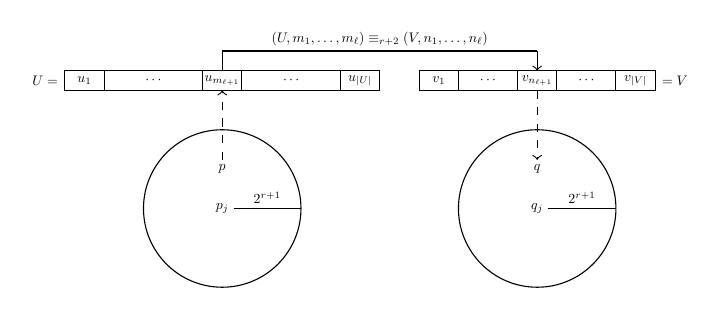
\begin{tikzpicture}[scale=0.5,every node/.style={scale=0.5}]
	 \draw (0,1) circle (2cm);
	 \draw (8,1) circle (2cm);
	 
	 \node (pj) at (0,1) {$p_j$};
	 \node (qj) at (8,1) {$q_j$};
	 \draw (pj) -- node[above] {$2^{r+1}$}  (2,1); 
	 \draw (qj) -- node[above] {$2^{r+1}$}  (10,1);
	 
	 \node (p) at (0, 2) {$p$};
	 \node (q) at (8, 2) {$q$};
	 
	 \path[draw] (-4, 4) rectangle (4,4.5);
	 \node at (-4.5, 4.25) {$U=$};
	 \draw (-3, 4) -- (-3, 4.5);
	 \draw (-.5, 4) -- (-.5, 4.5);
	 \draw (.5, 4) -- (.5, 4.5);
	 \draw (3, 4) -- (3, 4.5);
	 \node at (-3.5, 4.25) {$u_1$};
	 \node at (-1.75, 4.25) {$\cdots$};
	 \node at (0, 4.25) {$u_{m_{\ell + 1}}$};
	 \node at (1.75, 4.25) {$\cdots$};
	 \node at (3.5, 4.25) {$u_{|U|}$};
	 
	 \path[draw] (5, 4) rectangle (11,4.5);
	 \node at (11.5, 4.25) {$=V$};
	 \draw (6, 4) -- (6, 4.5);
	 \draw (7.5, 4) -- (7.5, 4.5);
	 \draw (8.5, 4) -- (8.5, 4.5);
	 \draw (10, 4) -- (10, 4.5);
	 \node at (5.5, 4.25) {$v_1$};
	 \node at (6.75, 4.25) {$\cdots$};
	 \node at (8, 4.25) {$v_{n_{\ell + 1}}$};
	 \node at (9.25, 4.25) {$\cdots$};
	 \node at (10.5, 4.25) {$v_{|V|}$};
	 
	 \draw[->, dashed] (p) -- (0, 4);
	 \draw[->, dashed] (8,4) -- (q);
	 
	 \path[draw] (0, 4.5) -- (0, 5) edge node[above] {$(U, m_1,\ldots, m_\ell) \equiv_{r+2} (V, n_1,\ldots,n_\ell)$} (8, 5) 
	                     (8, 5)            edge[->] (8, 4.5);
	              
	 
	\end{tikzpicture}
\end{center}